\section{自由度及刚体的自由度}\label{sec:10.01}

自由度就是描写体系几何位形所需的独立坐标的数目。譬如,
对于一个质点的直线运动,只需一个坐标x就完全确定了质点的位
置;对于一个质点的圆周运动,只需一个坐标$ \varphi $来确定质点的位
置(图\ref{fig:10.01})因此,这类运动的自由度是1。一般地说,质点
\begin{wrapfigure}[9]{r}{13em}
    \centering
    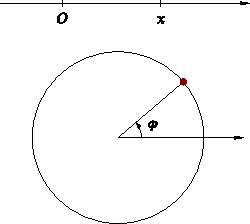
\includegraphics{figure/fig10.01}
    \caption{一维运动}
    \label{fig:10.01}
\end{wrapfigure}
的一维运动其自由度都是$ 1 $。对于
一个质点在三维空间中的运动,
需要三个独立坐标来描写它的位
置。可以用笛卡尔坐标$ x,y,z $
也可以用球极坐标$ r, \theta , \varphi $。因
此,质点是具有$ 3 $个自由度的物
理对象。

推广到由$ n $个质点构成的多
质点体系,一般说,如果要确定
体系的几何位形,就要$ 3 \times n $个坐标,即有$ 3n $个自由度。然而,在
某些情况下,由于质点之间存在确定的关系,故这$ 3n $个坐标并不
全是独立的。换言之,在质点体系中常存在着一些限制各质点自
由运动的条件。

例如,由两个质点$ m _ 1, m _ { 2 }  $ 构成的体系(图\ref{fig:10.02}),一般要用
% 286.jpg
$ 6 $个坐标$  \left( x _ { 1 } , y _ { 1 } , z _ { 1 } \right) ,\left(x_2,y_2,z_2\right) $如果两质点之间的距离是固
定的,其长度为$ r $,则上述$ 6 $个坐标之间有一个代数关系:
\begin{equation}\label{eqn:10.01.01}
    \left( x _ { 1 } - x _ { 2 } \right) ^ { 2 } + \left( y _ { 1 } - y _ { 2 } \right) ^ { 2 } + \left( z _ { 1 } - z _ { 2 } \right) ^ { 2 } = r ^ { 2 }
\end{equation}
\begin{wrapfigure}[7]{r}{9em}
    \centering
    
\includegraphics{figure/fig10.02}
    \caption{两质点体系}
    \label{fig:10.02}
\end{wrapfigure}
亦即只要知道了任何$ 5 $个坐标值,由上式
就完全确定了第$ 6 $个坐标的值。因此,独
立坐标的数目是$ 6-1=5 $,此体系的自由
度为$ 5 $。这种体系在自然界是有的,如
氢分子,它是由两个氢原子构成的,两原
子间的距离基本上可以认为是不变的。

再如,两个氢原子和一个氧原子组成
的体系。若三个原子是完全自由的运动,则有$ 9 $个自由度。如果

\begin{wrapfigure}[7]{l}{13em}
    \centering
    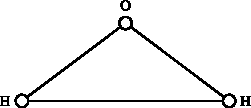
\includegraphics{figure/fig10.03}
    \caption{水分子的结构}
    \label{fig:10.03}
\end{wrapfigure}
\noindent
化合成水分子,两两之间的距离
不变,形成三角形(图\ref{fig:10.03}),则
描写三个原子位置的9个坐标应
满足$ 3 $个类似于式\eqref{eqn:10.01.01}的代
数关系。所以此时该体系的独立
坐标个数为$  9 - 3 = 6  $ ,即有$ 6 $个自
由度。

由四个原子组成的分子,例如NH\textsubscript{3},在化合之前,有$  3 \times 4 = 1 2  $
个自由度,化合成氨分子之后,形成如图\ref{fig:10.04}的四面体,两两原
子之间的距离都不变,共有$ 6 $个代数关系,所以这体系的自由度为
$ 1 2 - 6 = 6  $。

如果再增加一个原子,且它与原来四个原子的距离也都不变
(图\ref{fig:10.05})  ,则增加一个原子,就要增加$ 3 $个坐标,但同时却增加了
$ 4 $个代数关系式。要注意,新增加的$ 4 $个代数关系式并不是完全独
立的。因为在这$ 4 $个关系式中,任何$ 3 $个确定之后,第$ 4 $个也就确定
了。故仅有$ 3 $个新的独立代数关系式。因此,整个体系的自由度不
变仍然是$ 6 $。

% 287.jpg
\clearpage
\begin{figurex}
    \begin{minipage}[b]{0.5\linewidth}
        \centering
        
\includegraphics{figure/fig10.04}
        \caption{NH\textsubscript{3}的结构}
        \label{fig:10.04}
    \end{minipage}
    \begin{minipage}[b]{0.5\linewidth}
        \centering
        
\includegraphics{figure/fig10.05}
        \caption{五原子构成的体系}
        \label{fig:10.05}
    \end{minipage}
\end{figurex}

同理,我们可以推广到更多原子组成的分子,得到一个结论:
含有三个原子以上的分子,若原子不全处在一条直线上,则都有
$ 6 $个自由度。

把上述论断再作推广可以得到:由任意多个质点所构成的体
系,如果体系中所有质点之间的距离都是固定的,且不在一条直
线上,则体系的自由度必定是$ 6 $。这种多质点体系称为刚体。当
然,刚体的概念最早并不是从分子来的,而是来自于不变形的体
系。所谓不变形即组成体系的各质点之间相对位置在运动过程中
不发生变化。这种体系称为刚体,实际上,自然界中没有绝对的
刚体。刚体这一概念是一种理想化。只要可以忽略物体形变的影
响,则该物体就可以认为是刚体。